\documentclass[openany,a4paper,11pt]{kth-mag} % Remove open any before handing in
\usepackage[swedish,english]{babel}
\usepackage{textcomp}
\usepackage{lmodern}
\usepackage{graphicx}	
\usepackage{modifications}
\usepackage{algorithmicx}
\usepackage{amsmath}
\usepackage{amssymb}
\usepackage{algpseudocode}
\usepackage{hyperref}

% Todo:
% Fix width of pictures.
% Make a new roulette selection picture.
% Check that all references are used.
% Check that all figures are referred to.
% Check that the bibliography is consistent.
% Make sure hyphens are in all the correct places. See: http://oxforddictionaries.com/words/hyphen, e.g. decision-making
% All "section" should use small S.
% All "figure" should use large F.

\title{Evolution of Artificial Brains in Simulated Animal Behaviour}
\subtitle{Comparing radial basis, linear and random functions for decision-making}
\foreigntitle{Evolution av artificiella hj�rnor vid simulering av djurs beteende}
\author{Bj�rn Tegelund\\Johan Wikstr�m}
\date{November 2003}
\blurb{Bachelor's Thesis at CSC\\Supervisor: Petter �gren\\Examiner: M�rten Bj�rkman}
\trita{TRITA xxx yyyy-nn}
\begin{document}
\frontmatter
\pagestyle{empty}
\removepagenumbers
\maketitle
\selectlanguage{english}
\begin{abstract}
  Write this. % Write this

\end{abstract}
\clearpage
\begin{foreignabstract}{swedish}
  Skriv detta. % Write this

\end{foreignabstract}
\clearpage
\tableofcontents*
\mainmatter
\pagestyle{newchap}
\chapter{Introduction}

\section{Background}

% D�r s� �r relevant f�r uppgiften, visa viss medvetenhet om samh�lleliga och etiska aspekter, inklusive ekonomiskt, socialt och ekologiskt h�llbar utveckling.

Genetic algorithms are algorithms that emulate evolution in order to approximate an optimal solution to a problem. These algorithms have many uses and several natural evolutionary phenomena occur when using genetic algorithms as well. In nature, evolution has spawned a wide variety of survival strategies such as adaptation, camouflaging colours and mimicry. Genetic algorithms have been used on several occasions to simulate artificial life as well as artificial intelligence and this report is a continuation of that research. They have been used to train machine learning algorithms \cite{montana}, for robot motion planning \cite{huijsmann} and for the evolution simulator Gaia which utilises advanced genetic algorithms to train artificial neural networks \cite{gracias}. Artificial neural networks are commonly used machine learning algorithms for artificial intelligence. The results from Gaia showed several interesting behaviours, two prominent ones being searching for food and obstacle avoidance. Another study used artificial neural networks as a way to simulate camouflaging colours, using a more mathematical and controlled model \cite{holmgren}.

Since genetic algorithms emulate the natural process of evolution, several natural phenomena such as mimicry can be observed in genetic algorithms as well. This makes this group of algorithms especially suited for simulating populations of artificial animals, giving a very genuine impression of evolution. Since genetic algorithms are such a good metaphor for evolution in nature, they can be used to simulate natural evolution as well. The precision of the simulations depend on the ability to mimic evolution of traits and behaviours in nature.  Genetic algorithms provide a simplified model of these and makes it possible to analyse different evolutionary scenarios, including extremes that are uncommon in nature today, from different perspectives. The ability to accurately predict these scenarios becomes increasingly important as our environment becomes increasingly volatile. 

% Check this out: http://www.bbc.co.uk/news/science-environment-22039872 very current research, could be cool to refer to

\section{Scope and Objectives}

%In this report two simple forms of decision making models are implemented. Both are driven by genetic algorithms and both are compared to previous research on more advanced brain architechtures. Interesting patterns and phenomena are also recorded.

This report focuses on evolving simulated animal behaviour using two kinds of mathematical functions. As a baseline, a brain which makes random decisions is also used.  The genetic algorithms provide the genes which are used as input to the decision making models. Statistics such as learning speed, choice of strategy and how well the animals are able to adapt to their surroundings are then analysed. 

The animals will be given different tasks in each experiment including food gathering, predator avoidance and mimicking things in the world to survive. In each experiment the three decision making models are compared and contrasted. One goal of this project is to find out the advantages and disadvantages of both models, when used for simulating artificial intelligence.

Genetic algorithms have been used successfully in the past in similar experiments. In the Gaia report, the authors acknowledge that many of the behaviours observed could be implemented using simple linear associations \cite{gracias}. One of this project's goals is to determine which behaviours that can be observed using the simpler brain types - linear functions and radial-basis functions. 

% TODO: What did we manage to simulate?
%  Forcing them to adapt certain genetic phenomena such as adaptation (learning), co-evolution and extinction, mimicry, group forming and co-operation prioritised in the order presented (as increasingly complex behaviour and difficulty to simulate).

\section{Problem Statement}

\begin{enumerate}
\item Is it possible simulate evolution of animal behaviour using linear and radial-basis functions using genetic algorithms?
\item Are there any significant differences between the two contrasted decision making models?
\item Can any evolutionary phenomena from using genetic algorithms be observed in the simulated animals?
\end{enumerate}

\chapter{Technical Overview}

\section{Genetic Algorithms}

\subsection{Overview}
\label{ga_overview}

Genetic algorithms are a way of approximating solutions to NP-hard problems, a group of problems that are computationally expensive. They are a form of machine learning algorithms typically used to solve problems with a large or complex search space and where other machine learning algorithms fail \cite[p.~269-288]{marsland}. Genetic algorithms mimic natural selection in nature by defining a set of genomes, or individuals, where each genome represents a possible solution to the given problem. This genome is commonly stored as a string of 0:s and 1:s or as a list of floating point values. This set of genomes undergoes several iterations, or generations, of small improvements by fitness evaluation, selection, mutation and crossover. These operators all have equivalents in natural evolution and eventually the genomes will converge to a solution which represents a local minima in the search space. The advantage of genetic algorithms is that the crossover operator enables a wider search over the problem domain than many other approaches, using less calculations \cite{holland}. In the following subsections, the most crucial parts of the genetic algorithm will be explained and in figure \ref{algorithm-overview}   an overview of the genetic algorithm in pseudo code is depicted.

\begin{figure}
\begin{algorithmic}
\State $ S \gets $ a random distribution of genes
    \While {the genes have not converged towards a solution}

        \State $F\gets fitness(S)$
		\Comment Calculate fitness values for all $s \in S$
		\State $X \gets select(S,F)$
		\Comment Get a multiset of S using fitness values
		\State $C \gets crossover(X)$
		\Comment Apply crossover operator on multiset
		\State $M \gets mutate(C)$
		\Comment Apply mutation operator on crossed genes
		\State $S \gets M$
		\Comment Restart with the new generation
    \EndWhile
\end{algorithmic}
\caption{An overview of the genetic algorithm used in the experiments}
\label{algorithm-overview}
\end{figure}

\subsection{Fitness}
\label{ga_fitness}
Fitness is the only mean of measuring the success of the solution. In nature, fitness is simply determined by the number of offspring produced by the individual and the percentage of the offspring which survive long enough to generate new offspring\cite[p.~117]{darwin}. In 1932, Sewall Wright suggested that species adapt until they reach a local maxima in a fitness search space, which is a multidimensional space consisting of all possible combinations of genes and their resulting fitness. To reach another local maxima in the search space, which might be higher than the previous, the species must journey through a "valley" in the search space that would result in a temporarily lower fitness \cite{wright}. In genetic algorithms, the fitness function can be any value that describes each individual's success at solving the problem at hand. Genetic algorithms can get significant performance advantages by selecting the correct fitness function. The fitness function should be strictly positive for all inputs and preserve some form of relative internal ordering of the individuals. In most problems there are multiple choices of fitness functions and the best choice of fitness function is unique for every problem \cite[p.~272]{marsland}. For this reason, many different fitness functions were tried before settling for simply the life length of the individuals. Another reason for choosing this fitness function is that it is general, which allows the animals to freely choose strategies.

\subsection{Selection}
Selection is the process of selecting which organisms that should be allowed to reproduce and in what proportions. In nature, selection is closely tied to fitness, the fittest individual is also selected most often, but in genetic algorithms there are several different ways to model this selection process. A good fitness function should strike a balance between favouring the fittest individuals and allowing less fit individuals to survive in a reduced number.  One trivial selection function could be to simply select all individuals that pass a certain fitness threshold \cite[p.~273]{marsland}. This is a bad idea, however, since there are few ways to determine the correct threshold value. In the beginning of the evolution, a high threshold will exclude most of the genes due to low general fitness and this will lead to a fast reduction of genetic variation. In the later stages of the evolution all individuals will pass the threshold, rendering the selection function useless.

A better approach is the so called roulette wheel selection where each individual is mapped to an area of what looks like a roulette wheel, see figure \ref{roulettewheelpic}. A larger fitness value means a larger area on the roulette wheel and the selection function simply generates random values corresponding to the areas of this roulette wheel. In this way, the individuals are chosen based on a biased stochastic variable and there is room for individuals with high fitness to dominate as well as for individuals with low fitness to be included by chance. 

\begin{figure}
\centering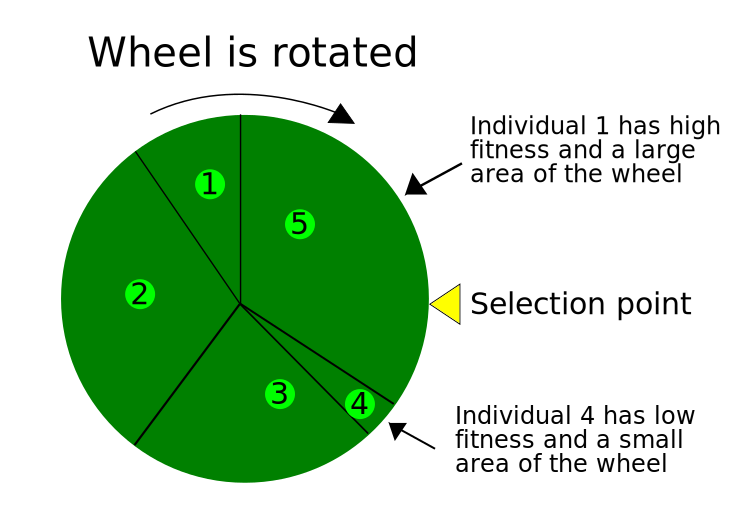
\includegraphics[scale=0.5]{roulette.pdf}
\caption{A visual representation of how the roulette wheel selection algorithm works.}
% Beh�ver vi source till detta? Hittades h�r: http://www.edc.ncl.ac.uk/highlight/rhjanuary2007g02.php/
% G�r om denna!
\label{roulettewheelpic}
\end{figure}
 
\subsection{Mutation}
\label{background_mutation}
Mutation is a random, usually small, change of an individual's genome. In nature this typically occurs spontaneously when new cells are formed and there are hundreds of factors which can induce mutation \cite[p.~46]{vij}. In genetic algorithms it is usually implemented as a small probability for each gene to mutate. When the genome consists of a series of 0:s and 1:s, the mutation operator is simply a flip of that bit and when the genes consist of floating point values, the mutation can be an addition or multiplication of a random value. If the mutation rate is too high, it becomes hard to reach convergence since the good solutions will often be mutated into worse solutions.

\begin{figure}
\centering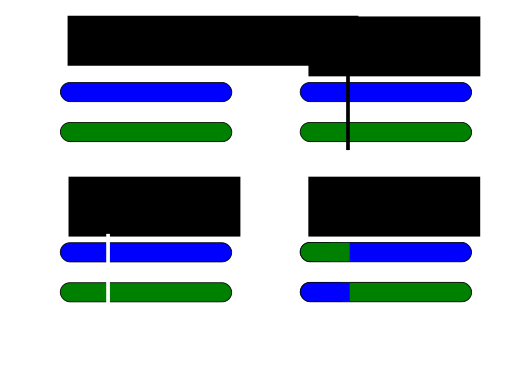
\includegraphics[scale=0.5]{crossover}
\caption{A schematic drawing showing single point crossover of two genomes.}
\label{crossover-figure}
\end{figure}

\subsection{Crossover}
Crossover is the operation of combining two genomes into two new genomes. One common crossover operator is known as  single point crossover and it consists of splitting two genomes at the same position and merging the split parts into two new genomes. The split position is chosen randomly and the two new genomes share no genes with each other. This process is displayed in Figure \ref{crossover-figure} There is also multiple point crossover where there are multiple splitting positions as well as uniform crossover where each gene can be exchanged with a certain probability.

\section{Evolutionary Concepts in Nature}
\subsection{Overview}
\label{evolutionary_overview}
This section provides a short overview of evolutionary concepts in nature which are mentioned in this report. As each individual solution the genetic algorithm proposes can be thought of as an individual in a population, many of the normal evolutionary phenomena can be observed in genetic algorithms as well.

\emph{Adaptation} is when an individual is forced to adapt to its surroundings in order to survive. In nature adaptation occurs over generations and the need to adapt is the primary motivator behind evolution \cite[p.~8]{king}. The fitness of an individual depends to a great extent on how well-adapted an individual is to its surroundings. In extreme environmental changes adaptation is typically accelerated and once the population can handle itself in the new environment smaller changes are made to meet secondary goals. A large population size increases the ability to adapt, as more smaller and potentially helpful adaptations can be made per generation. A smaller population is more unstable and vulnerable as random environmental changes can eradicate important individuals or genes from the population. An example of adaptation in nature is how the polar bear evolved to have thicker, whiter fur when moving to a colder, snow-covered environment.

\emph{Co-evolution} is when the evolution of a species is affected by the evolution of another \cite[p.~90]{king}. This could be both in a symbiotic, parasitic or a predator-versus-prey manner. When in a predator-versus-prey situation and the predator evolves faster, the prey is usually faced with extinction. If it is the other way around the predators are faced with extinction as they may not be able to catch enough prey for their population to survive. An example of this is how cheetah and its prey is in a constant battle of being able to run the fastest.

\emph{Mimicry} is a kind of adaptation where one species mimics another object's appearance or behaviour for protection \cite[p.~278]{king}. This could be camouflaging oneself as a stone or evolving brightly coloured patterns, characteristic of poisonous animals, despite not being poisonous in order to ward of potential predators. Mimicry can be found in certain species of butterflies which wings take on the shape, colour, and texture of leaves.

\section{Radial Basis Functions}
\subsection{Overview}

\begin{figure}
\centering\includegraphics[scale=0.5]{rbf_1d.png}
\caption{Three one-dimensional RBFs with varying $\mu$ and $\sigma$ values. $\mu$ determines the centre of the bell curve and $\sigma$ controls the slope of it.}
\label{3-RBF-functions}
\end{figure}

A radial basis function (RBF) is a bell-shaped function whose value depends on the distance from some centre \cite[p.~1-8]{buhmann}, as shown in Figure \ref{RBF-1}.  Radial basis functions are commonly used in artificial neural networks as a way to encode input information. They are favourable to use as they have locality, something which linear functions do not. Locality means that the function value is zero in almost the entire domain of the function. This is displayed in Figure \ref{3-RBF-functions}. This makes them useful for function approximation, as any function can be approximated as the sum of a number of weighted radial basis functions. Linear functions do not have this property. A property of radial basis functions which can both be interpreted as an advantage and disadvantage is that their value never exceeds a given constant, compared to a linear function which can grow to infinitely high or low numbers.

Radial basis functions are commonly implemented using a formula such as in Figure \ref{RBF-1}, which is a three-dimensional function centred around $(\mu _{x}$, $\mu _{y}$, $\mu _{z})$. The width of the bell-curve in each dimension is determined by $\sigma _{x}$, $\sigma _{y}$ and $\sigma _{z}$ respectively.

\begin{figure}
\begin{equation*}
f(x,y,z) = A_x*\exp(-\frac{(x-\mu_{x})^{2}}{2 \sigma _{x}^{2}}) + A_y*\exp(-\frac{(y-\mu_{y})^{2}}{2 \sigma _{y}^{2}}) + A_z*\exp(-\frac{(z-\mu_{z})^{2}}{2 \sigma _{z}^{2}})
\end{equation*}
\caption{A sum of three radial basis functions, corresponding to three input values.$A_x$, $A_y$ and $A_z$ lies within the interval $[-1,1]$ and ensures that $f(x,y,z)$ can be negative.}
\label{RBF-1}
\end{figure}

\chapter{Implementation}
\section{Model}
\begin{figure}
\centering\includegraphics[scale=0.5]{simulation.png}
\caption{A screenshot of the simulation, showing green plants(green circles), herbivores (multicoloured circels with antennae) and a predator(red circle with inner circle and antennae).}
\end{figure}
\subsection{Simulation in Python}
\label{simulation-in-python}
Python was chosen as the language to implement the simulation in as it is a high-level language suited for quickly building prototypes. It also has an abundance of third-party libraries which helps reduce implementation time significantly. A third-party library called DEAP (Distributed Evolutionary Algorithms in Python) was used for the evolutionary algorithms. DEAP proved to be flexible enough for the task as it allows the user to define their own selection, mutation and crossover algorithms as well as mixing them with the accompanying built-in algorithms. Pygame and Matplotlib were used for graphical rendering, Pygame for rendering the actual simulation and Matplotlib for producing graphs from the extracted data. To increase performance Pypy, Numpy and Python's built-in support for multiprocessing were used to decrease runtime significantly. For a comprehensive list of the tools used, please see Appendix \ref{list-of-third-party-tools}.

\subsection{Simulated World}
\label{simulated_world}
% Mention GitHub for exact values, different constants etc
These libraries were combined to create a model of the world in which the animals will be simulated. The world contains animals, which are spheres with two antennae protruding from their bodies at angles $\pi /6$ and $-\pi / 6$. There are two kinds of animals in the world; herbivores and predators. The herbivores' colours are decided by their genes. There may also be predators in the world that are similar to herbivores apart from that they consume different food and always have a strong red colour. While herbivores eat green plants, which are green circles placed randomly within the world, predators instead eat herbivores. To make things more difficult herbivores also have to avoid red plants, which are red circles. These represent "bad" or poisonous food. After a plant is eaten there is a small probability each tick that a new one will be placed into the world at a random location. As predators have no interest in eating plants they do not detect or have any consequences from colliding with plants. There are also walls around the border of the world which the animals cannot pass through. They are coloured blue in order for the herbivores to be able to make a clear distinction between walls, plants, predators and other herbivores. Collision and detection, which are the only ways of interaction between two objects, are governed by the following rules:

\begin{enumerate}
\item Interaction between two objects occur when they collide. A collision occurs when the distance between the centres of the two objects is smaller than the sum of their radii. Exactly what happens depends on the type of objects.
\item Detection occurs when an object crosses the antennae of either a herbivore or predator.
\end{enumerate}

At first each possible collision is checked and if one has occurred its effect is immediate. If a herbivore collides with a plant, that plant is eaten. If it is a green plant the herbivore's lifespan is increased slightly. If it is a red one the herbivore is killed. If a predator collides with a plant nothing happens and if it collides with a herbivore the herbivore is killed and the predator's lifespan is increased. After that a check for detection occurs and the animals which have detected objects are allowed to process the inputs and apply a $\Delta s$ and a $\Delta r$ (change in speed and rotation) to their current speed and rotation. Every animal is then moved in accordance with their speed and rotation. This decision process is described in sections \ref{decision_making} to \ref{random_decision_making}.

Due to performance issues all the animals are not present in the same simulation. Instead, parts of the populations are broken off and simulated separately and the results are then gathered and used to create the next generation. The reason behind this is that the detection and collision algorithms have a time-complexity of $O(n^{2})$ and therefore scale poorly. In practice this means that each simulation takes four times as long if the number of animals per simulation is doubled. By doing this trade-off where a lower number per simulation was used it was possible to run a higher number of iterations of the genetic algorithm in the same amount of time.

There are many specific constants which need to be fine-tuned for optimal results and performance, such as animal size, maximum speed and maximum life length among others. Listing all of these and their purpose would not contribute to this report, but the interested reader can find the entire source code for the project at the location specified in Appendix \ref{src_code}.

% Need to mention how new plants are spawned
% Mention ticks, how many ticks etc
% This section is a bit messy. It's difficult to describe all the mechanics of the world using small steps. 

\subsection{Methods of Enforcing Behaviour}

In order to investigate which natural evolutionary mechanisms could be observed when using genetic algorithms in this way it was necessary to find methods to enforce behaviour in the animals. 
It is also interesting to see which evolutionary strategies are favoured by the different brains when placed in particular situations. 
Methods of doing this could be adding additional inputs to the brains or adding extra terms in the calculations to allow the approximation of more complex functions and thus more complex behaviour. 
This approach does however come at the cost of computing power. 
For each gene added the expected time for convergence is increased. %Ref? 

To focus more on which natural evolution mechanisms occur, an approach was chosen which focused more on changing the animals' environment instead of the animals themselves. 
An example of an approach used was to add red plants into the world. 
The task of eating green plants then became much more difficult as the animals also had to avoid mistakingly colliding with red plants. 
Another addition which allowed for more dynamics in the world was the choice to allow the herbivores to have different colours which also depended on their genes. 
By doing this it enabled the use of the evolutionary strategy known as mimicry, described in Section \ref{evolutionary_overview}. % Could also refer to results here.

%Adding predators\\ % Not really mentioned

\subsection{Decision Making}
\label{decision_making}
All brains in our simulation have a similar structure, they are functions with eight inputs and two outputs. 
When input is received by an animal, it is in the form of eight numbers, four for each antenna. 
Three of the inputs for each antenna are the red-, green- and blue components of the currently detected object's colour. 
These inputs are normalised within the interval $[0,1]$. 
The fourth input is zero when no object is detected and one when an object is. 
It was deemed necessary to include the fourth input, saying if an object is detected or not, to avoid certain edge-cases.
For example, if an animal were to detect a black object this would be equal to detecting nothing at all if using only three inputs, which in turn would give no reaction.

The outputs produced from this consists of the values $\Delta r$ and $\Delta s$ which denotes change in rotation and change in speed. 
Both output values are normalised to the interval $[-1,1]$ to account for the possibilities of negative rotation and negative acceleration. 
These values are then translated into reasonable values in the simulation. 
The maximum acceleration is determined by the size of the animals, the size of the world and the maximum speed of the animals.
This enables scaling of the world without affecting the simulation itself, by tweaking those constants. 
The maximum allowed change in rotation is 180$^\circ$ or $\pi$ since the interval $[-\pi,\pi]$ covers the entire circle. 
A larger allowed change in rotation would have made learning harder as there would be multiple correct responses to a situation, e.g $\Delta r = v, \Delta r = v+ 2\pi, \Delta r = v+ 4\pi \dots $.

\subsection{Linear Decision Making}
\label{linear-decision-making}
The linear brain is a very simple model for artificial intelligence. 
There are twelve genes in total in the interval $[-1,1]$.
These genes correspond to three colours per antenna times two antennae times two outputs from the brain. 
Both $\Delta r$ and $\Delta s$ are calculated using the same method as mentioned previously.
%Ref?
In Figure \ref{linear-decide}, the first three components of the left and right antennae vectors, the ones containing the colour data, are called $\mathbf{x_{l}}$ and $\mathbf{x_{r}}$ respectively. 
The fourth components are called $l_4$ and $r_4$, and are the variables which show if an object has been detected or not.
There are twelve genes involved in total in the linear brain, six of them apply to this equation and they are divided into two vectors $\mathbf{g_{1-3}}$ and $\mathbf{g_{4-6}}$ using genes 1-3 and 4-6. 
The change in speed $\Delta s$ is calculated in the exact same way using the same inputs but genes 7-12 instead.

\begin{figure}
\begin{equation*}
\Delta r =
\begin{cases}
	0 																				& \text{if $l_4 = 0$ and $r_4 = 0$},\\
	S(\mathbf{g_{1-3}} \circ \mathbf{x_l}) 											& \text{if $l_4 \neq 0$ and $r_4 = 0$}\\
	S(\mathbf{g_{4-6}} \circ \mathbf{x_r}) 											& \text{if $r_4 \neq 0$ and $l_4 = 0$}\\
	S(\mathbf{g_{1-3}} \circ \mathbf{x_l} + \mathbf{g_{4-6}} \circ \mathbf{x_r} ) 	& \text{if $r_4 \neq 0$ and $l_4 \neq 0$}\\
\end{cases}	
\end{equation*}
\caption{The linear brain's decision formula for change of rotation $\Delta r$. $S$ corresponds to a sigmoid function described in Chapter \ref{linear-decision-making}.}
\label{linear-decide}
\end{figure}

In the equation a sigmoid function $S$ is used to limit the outputs to be within $[-1,1]$. 
The function $\frac{1}{1+e^{-x}} * 2 -1$ was chosen as sigmoid function but any function $f:x\rightarrow y, x\in [-6,6], y \in [-1,1]$ would have worked as the only concern was to limit the output range to $[-1,1]$. 
The sigmoid function was however used as linear behaviour, with a relatively high steepness, near $x=0$ was desired. 
That gives the best learning rate and a flatter curve at the extremes. 
An $x$ value near the extremes of $[-6,6]$ corresponds to radical behaviour such as turning 180$^\circ$ or accelerating rapidly and an $x$ value near 0 corresponds to making minor adjustments of speed and angle when encountering an object. 
A high $x$ value also corresponds to a very rare event occurring, namely that both antennae detect objects with high colour values, meaning that they are all near 1. 
As the objective was to train the animals to behave as rationally as possible to common events, the sigmoid function was chosen to slow down the learning rate of rare, extreme events and behaviours and accelerate the learning of commonly occurring events and behaviours.
This corresponds to $x$-values in the sigmoid far from zero and near zero, respectively.
In this way, the animals still have the ability to make strong reactions, e.g. turning 180$^\circ$ when seeing a predator, but learning focuses more on the interesting behaviours, namely in which direction to turn or in which direction to accelerate. 
The reason for not choosing a simpler function, such as $f(x) = x/6$, as a normalising function was that it would have slowed down learning considerably giving more extreme cases a larger effect than desired.

\subsection{RBF-Based Decision Making}

In RBF-based decision making, the three inputs to each antenna are used in the function displayed in Figure~\ref{3-RBF-functions}. 
For each antenna, $\Delta r$  and $\Delta s$ are computed by summing RBF function values and normalising them using the same function $S$ as in section~\ref{linear-decision-making}. 
As also mentioned in the same section, $\Delta r$ and $\Delta s$ are calculated separately using the same function and inputs but using different genes.

\begin{figure}
\begin{equation}
\Delta r =
\begin{cases}
	0 										&	\text{if $l_4 = 0$ and $r_4 = 0$},\\
	S(f(\mathbf{x_l})) 						&	\text{if $l_4 \neq 0$ and $r_4 = 0$}\\
	S(f(\mathbf{x_r})) 						&	\text{if $l_4 = 0$ and $r_4 \neq 0$}\\
	S(f(\mathbf{x_l}) + f(\mathbf{x_r})) 	&	\text{if $l_4 \neq 0$ and $r_4 \neq 0$}\\
\end{cases}	
\end{equation}
\caption{Calculating the $\Delta r$ using RBF functions. 18 genes are implicitly used, nine genes for $A$:s, $\sigma$:s and $\mu$:s in $f$ (see Figure~\ref{RBF-1}) using input $\mathbf{x_l}$ and nine for $\mathbf{x_r}$ }
\label{RBF-decide}
	\end{figure}

Each radial basis function has a $\sigma$ and a $\mu$ which are decided by the animals' genes. 
$\sigma$ and $\mu$ are in the ranges of $[0,1]$ and $[-1,1]$ respectively. 
An additional gene is also used to weight the output, which corresponds to $A$ in Figure~\ref{3-RBF-functions}. 
This is required to allow the otherwise always positive RBF-functions to produce negative values as well. 
This means that the RBF brain has a total of 36 genes which needs to be trained as compared to the linear brain which only had twelve genes.

The difference between using radial basis functions and linear functions is that there is a better ability to approximate any decision-making strategy using radial basis functions. 
For example, an RBF-based brain could make the distinction between different shades of green and thus react differently to them while a linear function could only decide if more green produces a stronger or weaker output.

\subsection{Random Decision Making}
\label{random_decision_making}
\begin{figure}
\begin{equation}
\Delta r = 
\begin{cases}
	0 		& 	\text{if $l_4 = 0$ and $r_4 = 0$},\\
	r \in U([s-1,1])		&	\text{otherwise}
\end{cases}
\end{equation}
\caption{Calculating $\Delta r$ using random brain and the same notation as in Figure \ref{linear-decide} and Figure \ref{RBF-decide}. $r$ is a random number with uniform distribution.} 
\label{random-decide}
\end{figure}

In random decision making, only the fourth input which denotes whether an object has been detected or not, is used. If an object has been detected a $\Delta r$ and a $\Delta s$ within $[-1,1]$ are selected randomly with uniform probability. The sigmoid function $S$, which is used with both other brain architectures, is not used in the random brain, as the random values which are produced can easily be manipulated to be within the intended interval. 

\subsection{Genetic Algorithm}

The implemented genetic algorithm was similar to the one described in section \ref{ga_overview}. 
The main difference is that a combination of selection methods are used. 
Instead of only applying roulette selection elitism is included as well. 
This means that 10\% of the next population are exact copies from this generation's population, selecting the individuals with highest fitness. The modified algorithm is depicted in Figure \ref{our_ga_overview}. 

Elitism is used as roulette selection is a highly probabilistic algorithm, and it is then possible that some individuals with high fitnesses are not selected for the next generation. Elitism prevents these individuals from disappearing from the population by guaranteeing their genes will survive until the next generation. Typically these also provide a stable max fitness for the population, as they are expected to perform equally well in the next simulation. It should however be noted that this is  not the case with the simulations used in this report, as both herbivore, plant, and predator placement are random.

% Should mention probabilities for each swap, and for applying crossover at all
The crossover algorithm used for the experiments is a modified version of the uniform crossover algorithm mentioned in section \ref{background_mutation}. 
The difference is that instead of probabilistically replacing each gene, a "region" of genes are replaced instead. 
The idea behind this is that when applying crossover to RBF-based brains and only $\mu$ or $\sigma$ are replaced for a certain RBF then the resulting fitness will likely be lower than any of the parents'. 
A region is therefore defined as a group of subsequent genes. 
For the RBF-based brains the size of these regions are three genes long as both a weight, $\mu$ and $\sigma$ are needed for each RBF, and only one gene long for the linear brains as they only require one gene per calculation. 
When crossover is applied, one calculation, i.e. a RBF or linear unit, for either speed or rotation and for either the left or right antenna is switched. % Could mention that we had to be careful when choosing crossover operator as they could give quite crazy results. This seemed like a safe bet

Mutator

\begin{figure}
\begin{algorithmic}
\State $S \gets$ a random distribution of genomes
\State $G \gets$ number of generations
    \For{$g \gets 1; g < G; g++$}
        \State $fitnesses \gets run\_simulations(S)$
	\Comment Simulates parts of $S$, collects result
	\State $couple\_fitnesses(S,fitnesses)$
	\Comment Associates a fitness value with an animal
	\State $B \gets select\_best(S, length(S)/10)$
	\Comment Select 10\% best genomes
	\State $R \gets select\_roulette(S, length(S) * 9/10)$
	\Comment Selects rest using roulette
	\For{$child1 \in R, child2 \in R$}
		\State $crossover(child1,child2)$
		\Comment Probabilistically applies crossover
	\EndFor
	\For{$mutant \in R$}
		\State $mutate(mutant)$
		\Comment Probabilistically mutates an individual
	\EndFor
	\State $S \gets B \cup N$
	\Comment Restart with the new generation
    \EndFor
\end{algorithmic}
\caption{An overview of the genetic algorithm used in the simulation}
\label{our_ga_overview}
\end{figure}

\section{Experiments}
\subsection{Finding and eating food}
\label{exp1_desc}
This experiment consists of placing herbivores with randomly initialised genes in a world with only green plants in it. 
The number of green plants is variable and the results are checked after 500 generations. 
The population size is 200 and split into groups of 20 individuals, which are simulated separately for each generation. 
In each simulation the herbivores and plants are placed randomly into the world, with the herbivores having a random initial rotation. 
This is to avoid learning fixed patterns, that is doing the same sequence of actions each simulation. 
The downside of this is that the fitness values are not guaranteed to increase each generation, instead a longer interval needs to be examined. 
The number of plants in the beginning of the simulation is zero, and the number of plants may never exceed a fixed limit. 
As described in section \ref{simulated_world}, a herbivore's life length is increased when eating a green plant and the fitness of a herbivore is its life length.

The purpose of this experiment is to see whether they are able to learn at all and how fast learning occurs. 
This will be an example of adaptation, as described in section \ref{evolutionary_overview}, where the herbivores need to adapt to their new surroundings. 
It is also interesting to see if any specific behaviours occur in order to eat as many plants as possible. 
The results from the linear, RBF-based, and random brains will be compared in order to see if there are any clear differences between them when running such a simple experiment. 
It is expected that both types of brains will perform well in this task, as the problem is easy and solvable using simple colour associations, as proposed in \cite{gracias}.

In theory, a valid strategy could be not reacting to plants at all. 
Simply accelerating to maximum speed and "combing" the world for plants by rotating randomly is a plausible strategy. According to \cite{gracias} a good strategy is to simply continue in the same direction and accelerate towards a plant when it is detected. 
Another strategy observed in the same paper was to follow the walls of the world.
Following the walls of the world can be a good strategy for poorly adapted individuals, since it provides an easy way to cover a large area and by chance encounter green plants.

\subsection{Avoiding bad food}
\label{exp2_desc}
This is a variation of the experiment described in the previous section, with the addition of red plants. 
Similar to the green plants, the number of red plants is zero at the beginning of the simulation and always below a fixed amount, and they are also spawned in random locations. 
A problem with this approach is that a herbivore may be placed on top of a red plant, or vice versa. 
Nothing is done to prevent this, as with a large enough population size this is negligible. 
Another issue with this is that red and green plants could be placed above, or near, each other in the world, thus making it difficult for the herbivores to eat the green plant, while avoiding the red plant. 
The expected result of this is a lower average fitness value, but the decision to allow this to happen was based on comparing the brain types and seeing if they would handle this case differently.

By adding red plants to the simulation the task of living as long as possible becomes more complex. 
It is no longer a valid strategy to randomly pick a direction to go in each time a wall is encountered and not reacting to the detected plants. 
There are essentially two strategies for coping with this; the first strategy is trying to avoid red plants as much as possible, and the second is to focus more on eating green plants than avoiding red ones. 

\subsection{Predators and prey}
\label{exp3_desc}
In this experiment predators are added into the world. 
As mentioned in section \ref{simulated_world}, the predators' objective is to eat herbivores. 
The predators have a strong red colour. 
This is due to the fact that the prey are already learning to avoid red plants and if the predators are red as well it will be easier for them to avoid getting eaten. 
Due to the limitations of the linear brains, the RBF-based brains could have an unfair advantage if the predators could have multiple colours.
As the world is now it is beneficial to be able to treat blue, green, and red objects differently, and if the colours are mixed it quickly becomes too difficult for the linear brains to handle, as their reactions are a sum of the reactions to the individual components of the colour. 

In previous experiments there is no benefit in changing colour for the herbivores. 
In this experiment, however, it may be beneficial to try to mimic either predators or walls. 
When this phenomena occurs in nature it is known as mimicry and described in section \ref{evolutionary_overview}. 
Another interesting evolutionary phenomena which could occur is co-evolution. 
In this simulation that could mean the predator's average fitness continuously increasing while the herbivores' fitness slowly decreases, or vice versa, if the herbivores become proficient at avoiding predators.

\chapter{Results}
\section{Simulation results}
\subsection{Finding and eating food}
\label{exp1_res}
After running the first experiment the conclusion can be drawn that the genetic algorithm is able to train the herbivores to eat plants. Compared to the random brain, they perform about 125\% better after training for 300 generations. 
Most of the increase in fitness did occur between generations 1 and 100, as seen in Figure \ref{exp1_fitness}. 
The differences between the fitnesses of the linear and RBF-brains are small, which could be attributed to the randomness in the experiments and the simplicity of the given task. 
As expected in section \ref{exp1_desc}, there were mainly two prevalent food eating strategies during the experiments, namely following the walls of the world while looking for nearby food and the strategy of abruptly rotating in towards the centre of the world when encountering a wall. 
In all cases the herbivores accelerated and turned towards the green plants, just as expected in section \ref{exp1_desc} and mentioned in \cite{gracias}. % Max, avg, min fitness picture for this

\begin{figure}[htbp]
   \centering
   \includegraphics[scale=0.7]{exp1_fitness.png}
   \caption{A comparison between the average fitnesses of the RBF-based, linear and random brains when tasked only with eating green plants, according to section \ref{exp1_desc}.}
   \label{exp1_fitness}
\end{figure}

\begin{figure}[htbp]
   \centering
   \includegraphics[scale=0.7]{exp1_linearfitness.png}
   \caption{A graph showing the minimum, average and maximum fitness per generation for a simulation using linear brains and only green plants, as described in section \ref{exp1_desc}.}
   \label{exp1_linearfitness}
\end{figure}

A population size of 200 was an adequate amount as it provided a large enough genetic diversity within the population and small enough to be computationally cheap. 
High genetic diversity means a higher probability of initialising an individual with relatively successful genes, thus making the initial evolution faster. 
When using smaller population sizes the population and associated fitness values became more unstable and vulnerable to small random occurrences, such as a successful individual being randomly placed in a bad starting position. 
This can be related back to nature as an example of how smaller populations are unstable and more vulnerable, as stated in section \ref{evolutionary_overview}.

The minimum and maximum fitness values for each generation were also of interest. 
As each individual is given a base life length the minimum fitness never went below 100. 
It was also seldom higher than 100, which is due to the large population size and scarcity of plants in the world. 
The result of this is that there is almost always at least one unfit individual who will not eat a single plant for every generation. 
The maximum fitness reaches the theoretical maximum after only a few generations, as shown in Figure \ref{exp1_linearfitness}. 
This means that one or several herbivores have survived the full length of the simulation.
This could be a problem if a large share of the herbivores reach the maximum, since these individuals have the same fitness, but the average is low enough for this to not be a problem.
The average fitness increases steadily before reaching a plateau. 
The linear brains reached this plateau faster than the RBF-based brain, which could be an example of the longer convergence time for a higher number of genes.
This plateau represents a local maxima in the fitness search space, as mentioned in section \ref{ga_fitness}. 
The likelihood of this local maxima being the global maxima is increased as both the linear and RBF-based brains reach the same maxima.  % Are the large peaks in maximum fitness less common later in the simulation? This could be due to the fact that the herbivores become more intelligent and its not possible to be that much better than average.
% Could calculate theoretical maximum fitness

The colours of the herbivores converged to a random point which reflects the decreasing genetic diversity within the population. 
All brains showed these tendencies in this experiment, which was expected, as there is no advantage or disadvantage associated with a certain colour in this experiment.
An example of how the colours varied during the experiment can be found in Figure \ref{exp1_colour}.

\begin{figure}[htbp]
   \centering
   \includegraphics[scale=0.7]{exp1_colour.png}
   \caption{A graph over the change in the red, green, and blue components of the herbivores' colours during the experiment for the RBF-based brains with only green plants, according to section \ref{exp1_desc}.}
   \label{exp1_colour}
\end{figure}

%Can they learn at all?\\
%Increased life length desired\\
%How much better than random\\
%RBF vs Linear, learning rate, maximum average fitness\\
%Food eating strategies\\
%Population size, lowest possible, higher makes it more probable to have a successful randomly initialised individual\\
%Minimum fitness almost never goes over 0\\
%Maximum almost never reached ceiling\\
%Adaptation 1. Finding and eating food\\�

\subsection{Avoiding bad food}
Difference in strategies between linear and RBF brains\\
Comparison against random brains\\
Comparison between RBF and linear\\
Colours still converge to random point\\
Difference in average fitness against first experiment\\
Adaptation 2. Finding and eating food, avoiding "bad" food\\

\subsection{Predators and prey}
In the simulation when only predators, herbivores and green plants were present the predators dominated. 
They achieved high fitness values and suppressed the herbivores' average fitness. 
Where in section \ref{exp1_res}, with only herbivores and green plants, they had a fitness increase of about 125\% they were only able to increase their fitness by 70\% at most for linear brains and 50\% at most for RBF-based brains. 
Signs of an evolutionary arms-race have been found where spontaneous changes in colours triggered a decrease in number of herbivores killed by predators, as shown in Figure \ref{exp3_lineardbp}. 
This in turn leads to the predators adapting to the herbivores' new colour, and again increasing the ratio of herbivores killed by predators. 
The arms-race was not as apparent with the RBF-based brains, which is believed to be due to the locality property of the radial basis functions. This locality means that a small change in colour can still give the same, or a highly similar, reaction.

In the case of the RBF-based herbivores, the lack of major improvement is believed to be caused by the predators dominance which suppresses further development. 
This is an example of where genetic algorithms do not perform well, as the vast majority of the herbivores receive a low fitness value as they are eaten by predators and thus makes selection difficult. 
In almost every generation there are a few unlucky herbivores which are eaten by predators early in the simulation, and there are a few luckier individuals who manage to gather plants while the predators are busy chasing other herbivores. If a population of predators had had this kind of dominance over a population of prey in nature, the prey would likely be extinguished. However, due to the genetic algorithm the population survives and experiences the same scenario each generation.

\begin{figure}[htbp]
   \centering
   \includegraphics[scale=0.7]{exp3_lineardbp.png}
   \caption{
   A graph showing the herbivores' death-by-predator percentage when using linear brains, according to the specification in section \ref{exp3_desc}. Decreases in the percentage correlate to sudden changes in the herbivores' colour.}
   \label{exp3_lineardbp}
\end{figure}

Comparison between RBF and linear\\
%Random brained predators\\
Adding red plants to the mix\\
Strategies, look at death by predator graphs etc\\
%Colours\\
Evolutionary mechanisms\\
Co-evolution and extinction 1. Predator vs prey, prey eats food as in first experiment.\\
Mimicry 1. Making the prey mimic walls or predators to avoid being eaten.\\

\section{Discussion}
\subsection{Constraints and problems}
One serious and unexpected constraint was the performance of our algorithm. 
After profiling the code, several improvements were made. 
The main problem was the matching algorithms which compared all animals and plants to each other to determine collisions and detections. 
Checking all members of a list towards themselves is an operation which takes the time $O(n^2)$ on the size of the list and this is unacceptable as $n$ grows. 
The solution was to split up the population into several subpopulations as mentioned in section \ref{simulation-in-python} and run their simulation separately, sequentially or in parallel. 
This trick reduces the time complexity to $O(K*n)$ where $K$ is a constant.

The algorithms for collisions and detections were also scrutinised and all floating point calculations were replaced with pre-calculated values wherever possible. 
After the discovery of the scalar dot product as a big consumer of computation time, an alternative implementation was developed using pre-calculated values which sacrificed some memory and accuracy to achieve better running times. 
The standard Python implementation was also deemed too slow and PyPy, a fast Just-In-Time compiler was used to run the code for most of the time. 
Finally, multiple cores were utilised by using Python's built-in support for multiprocessing. 
Python was chosen over C++ since Python allows for a much faster development process which made this project feasible given the allotted amount of time.

Performance problems\\
Few runs of each experiment due to time constraints\\
Other unexpected problems?\\

\subsection{Simulation Accuracy and Application}

Highly simplified model, no flockbeteende, few predators\\
Useful as it shows that neural networks aren't always needed\\
Does show the phenomena which were sought after, but there are many more in nature\\
More useful for looking at specific aspects of evolution than a general simulation\\
Interesting as it combines results from holmberg and gracias\\
Antennae model is not realistic, can not see in front of them or more than 1 thing per eye\\
Herbivores would most likely notice being chased\\

\section{Conclusions and Future Work}

\begin{thebibliography}{99}
% We are using the APA style of referencing

\bibitem{montana} 
Montana, D. J.,  and Davis, L. (1989, August). Training feedforward neural networks using genetic algorithms. In \emph{Proceedings of the eleventh international joint conference on artificial Intelligence} (Vol. 1, pp. 762-767).
\bibitem{gracias}
Gracias N., Pereira H., Lima J.A., Rosa A. (1997). Gaia: An Artificial Life Environment for Ecological Systems Simulation \emph{Artificial Life V: Proceedings of the Fifth International Workshop on the Synthesis and Simulation of Living Systems} (Vol. 5). Mit Press.
\bibitem{marsland}
Marsland, S. (2009). \emph{Machine Learning, an Algorithmic Perspective}. CSC-Press
\bibitem{holland}
Holland, J. H. (1992). Genetic algorithms. \emph{Scientific american, 267(1)} (pp. 66-72).
\bibitem{buhmann}
Buhmann, M. D. (2003) \emph{Radial Basis Functions: Theory and Implementations}. Cambridge University Press
\bibitem{darwin}
Darwin, C, (1861) \emph{On the origin of species by means of natural selection; or, The preservation of favoured races in the struggle for life}. D. Appleton and Company
\bibitem{vij}
Vij, K. and Biswas, R. (2004) \emph{Basics of DNA \& Evidentiary Issues}. Jaypee Brothers Publishers
\bibitem{huijsmann}
Huijsmann, R., Haasdijk E., Eiben A. E. (2012) An On-line On-board Distributed Algorithm for Evolutionary Robotics. In \emph{Artificial Evolution} (pp. 73-84). Springer Berlin Heidelberg
\bibitem{wright}
Wright, S., (1932), The Roles of Mutation, Inbreeding, Crossbreeding and Selection in Evolution. In \emph{Proceedings of the Sixth International Congress on Genetics} (pp. 355-366). Brooklyn Botanic Garden % Refer to this one when discussing fitness landscape. Sewall Wright proposed that populations occupy adaptive peaks on a fitness landscape. In order to evolve to another, higher peak, a population would first have to pass through a valley of maladaptive intermediate stages.[65] A given population might be "trapped" on a peak that is not optimally adapted.
\bibitem{king}
King, R. C., Stansfield W. D., Mulligan, P. K., (2006) \emph{A Dictionary of Genetics}. Oxford University Press
\bibitem{holmgren}
Holmgren, N. M. A., Enquist, M., (1999) Dynamics of mimicry evolution. In \emph{Biological Journal of the Linnean Society}, issue 66 (pp. 145-158). Wiley Online Library
\end{thebibliography}

\listoffigures
\emph{Note:} all of the figures have been created by the authors.

\appendix
\addappheadtotoc
\chapter{Third-party libraries and tools used}
\label{list-of-third-party-tools}
\begin{itemize}
\item DEAP - Distributed Evolutionary Algorithms in Python \url{http://deap.gel.ulaval.ca/doc/default/index.html}
\item PyPy - A fast Just-in-Time compiler for Python. \url{http://pypy.org/}
\item Pygame - A computer game and visualisation package for python. \url{http://www.pygame.org/docs/}
\item NumPy - A Python package for numerical calculations. \url{http://www.numpy.org/}
\item matplotlib - A Python package for rendering graphs. \url{http://matplotlib.org/}
\end{itemize}

\chapter{Source Code}
\label{src_code}
The source code used to generate all of the results can be found at: % Remember to make a clone of the GitHub code and host it as public.

\chapter{Statement of Collaboration}
Both authors have spent an equal amount of time working on and contributing to the code, experiments and this report.

\end{document}
